\subsection{Porous medium}

The Theory of Mixtures as one of the basic approaches to model the complex behavior of porous media has been developed (concerning basic assumptions see e.g. \cite{Bow:1976,TT:1960}). As the Theory of Mixtures does not incorporate any information about the microscopic structure of the material\footnote{Within the context of the Theory of Mixtures the ideal mixture of all constituents of a multiphase medium is postulated. Consequently, the realistic modeling of the mutual interactions of the constituents is difficult.}, it has been combined with the Concept of Volume Fractions by e.g. \cite{Bow:1980,BE:1986a,LS:1998,Pre:1980}. Within the context of this enhanced Theory of Mixtures (also known as Theory of Porous Media), all kinematical and physical quantities can be considered at the macroscale as local statistical averages of their values at the underlying microscale.
%
Concerning a detailed overview about the history of the modeling of the behavior of multiphase multicomponent porous media, the reader is referred to e.g. \cite{Boer:2000}. Comprehensive studies about the theoretical foundation and numerical algorithms for the simulation of coupled problems of multiphase continua are given in e.g. \cite{Boer:2000,EB:2002,LS:1998} and the quotations therein. 

\vspace{4cm}
\begin{figure}[htbp]
\hspace{3cm}
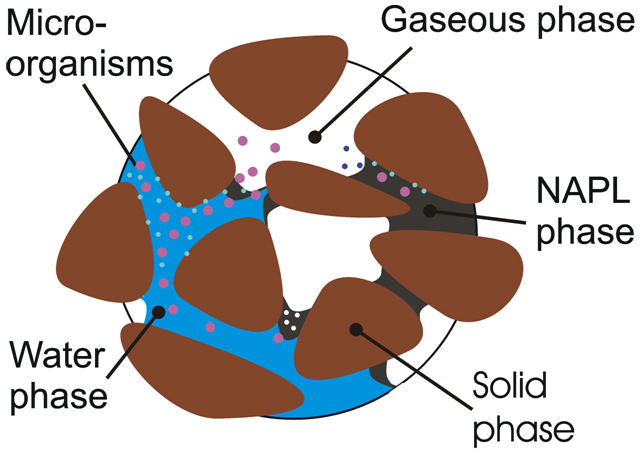
\includegraphics[width=0.06\columnwidth]{figures/pm.png}
\caption{Conceptual approach of a porous medium model}
\label{fig:pm1}
\end{figure}

The individual constituents $\varphi^{\alpha}$ of a porous material represent the phases of the overall aggregate or components within a phase. Below, $\alpha=s$ marks one immiscible solid phase (no sorption processes are considered), and $\alpha=\gamma$ denote several immiscible pore fluid phases. 
%
A porous medium, however, consists of multiple phases (fluids such as water, air and non-aqueous phase liquids (NAPLs) as well as solids). 
Moreover, these phases can contain several chemical components which can be dissolved in liquids or adsorbed to the solid phase (Fig. \ref{fig:pm1}).

Within the framework of the Concept of Volume Fractions, scalar variables like volume fractions and saturations are defined to describe the microstructure of a porous medium in a macroscopic manner neglecting the real topology and distribution of the pores. These variables serve as measures of local fractions of the individual constituents. The volume fractions $n^{\alpha}$ represent the ratio of the partial volume $dv^{\alpha}$ of a given constituent $\varphi^{\alpha}$ of a multiphase body with respect to the overall volume $dv$ of a representative elementary volume (REV) of the control domain $\Omega$ under consideration. Consequently, based on the definitions of the overall volume of the control domain
\begin{equation}
V=\int\limits_{\Omega}\,dv
\label{eq1}
\end{equation}
and the corresponding partial volumes of the individual constituents
\begin{equation}
V^{\alpha}=\int\limits_{\Omega}\,dv^{\alpha}\qquad\mbox{with}\qquad V=\sum\limits_{\alpha}\,V^{\alpha}
\label{eq2}
\end{equation}
the volume fractions
\begin{equation}
n^{\alpha}=\frac{dv^{\alpha}}{dv}
\label{eq3}
\end{equation}
provide some information about the local volume distribution of the individual constituents.
\begin{equation}
V^{\alpha}=\int\limits_{\Omega}\,dv^{\alpha}=\int\limits_{\Omega}\,n^{\alpha}\,dv
\label{eq4}
\end{equation}
One of the most characteristic media properties of a porous material is the porosity, the local amount of fluid volume fractions.
\begin{equation}
n=\sum\limits_{\gamma}\,n^{\gamma}=1\,-\,n^s
\label{eq5}
\end{equation}
Since, in general, the overall medium is completely filled with matter, from Eqn.~(\ref{eq2}) follows the saturation condition regarding the overall aggregate.
\begin{equation}
\sum\limits_{\alpha}\,n^{\alpha}=1
\label{eq6}
\end{equation}

If multiphase flow occurs, it is more convenient for various applications to use the (partial) fluid saturations $S^{\gamma}$ instead of the volume fractions. These local functions are given by
\begin{equation}
S^{\gamma}=\frac{dv^{\gamma}}{dv-dv^s}=\frac{n^{\gamma}}{n}
\label{eq7}
\end{equation}
obviously fulfilling the saturation condition regarding the pore content.
\begin{equation}
\sum\limits_{\gamma}\,S^{\gamma}=1
\label{eq8}
\end{equation}

Usually, constraint conditions addressing real physical effects are formulated to simplify complex mathematical and numerical models. Within the context of porous media, it is reasonable in most applications to assume the (material) incompressibility of constituents as a substantial constraint condition. The issue of (in)compressibility of a material is closely connected to the possible temporal evolution of its mass density.

Within the framework of the Concept of Volume Fractions, two different formulations of mass density related to the constituents of a porous medium are introduced. The so-called material (effective, realistic) density $\rho^{\alpha R}$ is defined as the ratio of the mass fraction $dm^{\alpha}$ of the given individual constituent $\varphi^{\alpha}$ with respect to its partial volume fraction.
\begin{equation}
\rho^{\alpha R}=\frac{dm^{\alpha}}{dv^{\alpha}}
\label{eq9}
\end{equation}
In contrast, the so-called partial (global, bulk) density is given by the ratio of the mass fraction of the constituent under consideration with respect to the volume fraction of the overall aggregate.
\begin{equation}
\rho^{\alpha}=\frac{dm^{\alpha}}{dv}
\label{eq10}
\end{equation}
Based on the definition of the volume fractions (\ref{eq3}), the material and the partial densities are correlated to each other.
\begin{equation}
\rho^{\alpha}=n^{\alpha}\,\rho^{\alpha R}
\label{eq11}
\end{equation}
If the volume fractions change with time under external loading, from Eqn.~(\ref{eq11}) follows that for an intrinsically incompressible individual constituent (constant material mass density) compressibility referred to the overall aggregate is observed.
\begin{equation}
\rho^{\alpha R}=\mbox{const} \quad\Rightarrow\quad
\rho^{\alpha}\,\neq\,\mbox{const}\quad\mbox{as}\quad n^{\alpha}\,\neq\,\mbox{const}
\label{eq12}
\end{equation}

Obviously, the mass density of the porous medium (homogenized overall aggregate) is defined as the sum of the partial densities of its constituents.
\begin{equation}
\rho=\sum\limits_{\alpha}\rho^{\alpha}
\label{eq13}
\end{equation}

The conceptual idea behind the formulations and relations presented above consists in the assumption that the mass fractions of all constituents of the multiphase medium are simultaneously present and statistically uniformly distributed over the entire control domain. Within this context, the material body under consideration is theoretically substituted by an aggregate completely and continuously filled by superimposed (overlapping) homogenized partial continua. In other words, all constituents of a porous medium are characterized as smeared substitute continua with reduced mass densities. Consequently, the motion and physics of the individual constituents as well as the overall aggregate can be specified by well-accepted phenomenological methods of continuum mechanics.

Describing the transport and deformation of the constituents of porous media within the framework of continuum mechanics it is assumed that the geometry of the control domain under consideration is characterized at each time by the solid skeleton, whereas the fluid pore content is able to flow across the boundary of the surface. This assumption serves as conceptual nucleus for the simulation of complex, coupled physical processes in multiphase porous media, particularly if a deformable solid skeleton is observed. Within this context, it proves to be reasonable not to model the absolute motion state of the pore content, but its motion relative to the motion of the solid phase, considering the porous medium as a local thermodynamic open system with the solid skeleton as volume under observation.

The macroscopic characterization of the physical processes considering the real microstructural situation in a statistically averaged manner is completely adequate for the most engineering, geotechnological and biomechanical problems under consideration (cf. \cite{GWASG:2006} and others).